A Resnet50 iteratív tanításának eredményei négy lépésben először 1000 majd 5000 azután 10000 végül pedig 25000 képes halmazon. Ezelet a lépéseket 1k, 5k 10k 25k rövidítésekkel fogom jelölni.

%1K-----------------------------------------------------------------------------
\subsubsection{1k adathalmazon történő tanítás lépései Resnet50 modellen.}
  \begin{itemize} 
    \item Epoch 1/10 - train: 15/15 [00:06<00:00, 2.15it/s]
    \item Epoch 1: Train loss=4.7268, acc=0.0143 Val loss=4.6176, acc=0.0545
    \item Epoch 2/10 - train: 15/15 [00:04<00:00, 3.13it/s]
    \item Epoch 2: Train loss=4.2507, acc=0.4265 Val loss=4.3277, acc=0.1355
    \item Epoch 3/10 - train: 15/15 [00:04<00:00, 3.12it/s]
    \item Epoch 3: Train loss=3.6435, acc=0.7050 Val loss=3.9273, acc=0.1929
    \item Epoch 4/10 - train: 15/15 [00:04<00:00, 3.10it/s]
    \item Epoch 4: Train loss=2.9406, acc=0.8432 Val loss=3.6216, acc=0.2660
    \item Epoch 5/10 - train: 15/15 [00:04<00:00, 3.10it/s]
    \item Epoch 5: Train loss=2.2647, acc=0.9090 Val loss=3.3172, acc=0.2780
    \item Epoch 6/10 - train: 15/15 [00:04<00:00, 3.09it/s]
    \item Epoch 6: Train loss=1.6587, acc=0.9178 Val loss=3.0913, acc=0.3027
    \item Epoch 7/10 - train: 15/15 [00:04<00:00, 3.05it/s]
    \item Epoch 7: Train loss=1.1541, acc=0.9561 Val loss=2.8877, acc=0.3070
    \item Epoch 8/10 - train: 15/15 [00:04<00:00, 3.07it/s]
    \item Epoch 8: Train loss=0.7962, acc=0.9792 Val loss=2.8046, acc=0.3179
    \item Epoch 9/10 - train: 15/15 [00:04<00:00, 3.08it/s]
    \item Epoch 9: Train loss=0.5309, acc=0.9912 Val loss=2.7045, acc=0.3295
    \item Epoch 10/10 - train: 15/15 [00:04<00:00, 3.07it/s]
    \item Epoch 10: Train loss=0.3352, acc=0.9967 Val loss=2.7344, acc=0.3036
  \end{itemize}

\subsubsection{1k adathalmazon történő tanítás grafikonja Resnet50 modellen.}
  \begin{figure}[H]
    \centering
    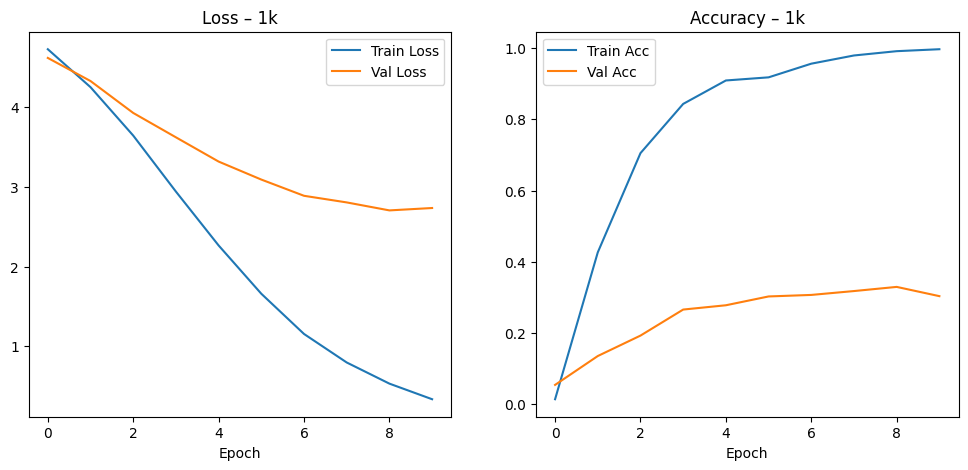
\includegraphics[width=1.0\textwidth]{images/phase03/phase03_ResNet50_1K_learning_curve.png}
    \caption{1k adathalmazon történő tanítás grafikonja Resnet50 modellen.}
    \label{fig:phase03_ResNet50_1K_learning_curve}
  \end{figure}

  \subsubsection{1k adathalmazon történő tanítás eredményei.}
  \begin{center}
    \begin{longtable}{l c}
    \caption{1k tanítás ResNet50-en.} \label{tab:phase03_ResNet50_1k} \\
    \toprule
    \textbf{Metrika} & \textbf{Érték} \\
    \midrule
    \endfirsthead
    \toprule
    \textbf{Metrika} & \textbf{Érték} \\
    \midrule
    \endhead
    Top-1 Accuracy & 0.3022 \\
    Top-5 Accuracy & 0.6505 \\
    Precision      & 0.2851 \\
    Recall         & 0.3149 \\
    F1-score       & 0.2820 \\
    Inference time & 31.49 sec \\
    \bottomrule
    \end{longtable}
  \end{center}


%5K-----------------------------------------------------------------------------
\subsubsection{5k adathalmazon történő tanítás lépései Resnet50 modellen.}
  \begin{itemize} 
    \item Epoch 1/10 - train: 77/77 [00:25<00:00,  3.07it/s]
    \item Epoch 1: Train loss=4.2541, acc=0.1336 Val loss=2.9191, acc=0.3120
    \item Epoch 2/10 - train: 77/77 [00:25<00:00,  3.08it/s]
    \item Epoch 2: Train loss=2.4980, acc=0.4419 Val loss=2.2629, acc=0.4149
    \item Epoch 3/10 - train: 77/77 [00:25<00:00,  3.08it/s]
    \item Epoch 3: Train loss=1.5075, acc=0.6589 Val loss=2.1996, acc=0.4065
    \item Epoch 4/10 - train: 77/77 [00:25<00:00,  3.07it/s]
    \item Epoch 4: Train loss=0.8867, acc=0.8315 Val loss=2.0922, acc=0.4397
    \item Epoch 5/10 - train: 77/77 [00:25<00:00,  3.08it/s]
    \item Epoch 5: Train loss=0.4669, acc=0.9247 Val loss=2.0961, acc=0.4400
    \item Epoch 6/10 - train: 77/77 [00:25<00:00,  3.08it/s]
    \item Epoch 6: Train loss=0.2292, acc=0.9753 Val loss=2.0989, acc=0.4490
    \item Epoch 7/10 - train: 77/77 [00:25<00:00,  3.07it/s]
    \item Epoch 7: Train loss=0.1167, acc=0.9914 Val loss=2.1723, acc=0.4536
    \item Epoch 8/10 - train: 77/77 [00:25<00:00,  3.08it/s]
    \item Epoch 8: Train loss=0.0653, acc=0.9955 Val loss=2.1871, acc=0.4492
    \item Epoch 9/10 - train: 77/77 [00:25<00:00,  3.07it/s]
    \item Epoch 9: Train loss=0.0356, acc=0.9988 Val loss=2.2443, acc=0.4525
    \item Epoch 10/10 - train: 77/77 [00:25<00:00,  3.08it/s]
    \item Epoch 10: Train loss=0.0250, acc=0.9992 Val loss=2.2541, acc=0.4598
  \end{itemize}

\subsubsection{5k adathalmazon történő tanítás grafikonja Resnet50 modellen.}
  \begin{figure}[H]
    \centering
    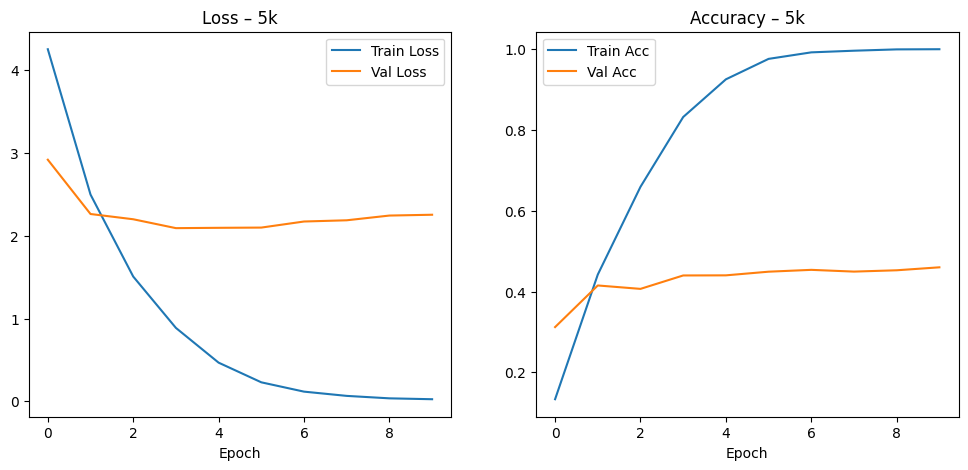
\includegraphics[width=1.0\textwidth]{images/phase03/phase03_ResNet50_5K_learning_curve.png}
    \caption{5k adathalmazon történő tanítás grafikonja Resnet50 modellen.}
    \label{fig:phase03_ResNet50_5K_learning_curve}
  \end{figure}


\subsubsection{5k adathalmazon történő tanítás eredményei.}
  \begin{center}
    \begin{longtable}{l c}
    \caption{5k tanítás ResNet50-en.} \label{tab:phase03_ResNet50_5k} \\
    \toprule
    \textbf{Metrika} & \textbf{Érték} \\
    \midrule
    \endfirsthead
    \toprule
    \textbf{Metrika} & \textbf{Érték} \\
    \midrule
    \endhead
    Top-1 Accuracy & 0.4603 \\
    Top-5 Accuracy & 0.7766 \\
    Precision      & 0.4254 \\
    Recall         & 0.4762 \\
    F1-score       & 0.4325 \\
    Inference time & 31.72 sec \\
    \bottomrule
    \end{longtable}
  \end{center}

%10K-----------------------------------------------------------------------------
\subsubsection{10k adathalmazon történő tanítás lépései Resnet50 modellen.}


\subsubsection{10k adathalmazon történő tanítás grafikonja Resnet50 modellen.}
  \begin{figure}[H]
    \centering
    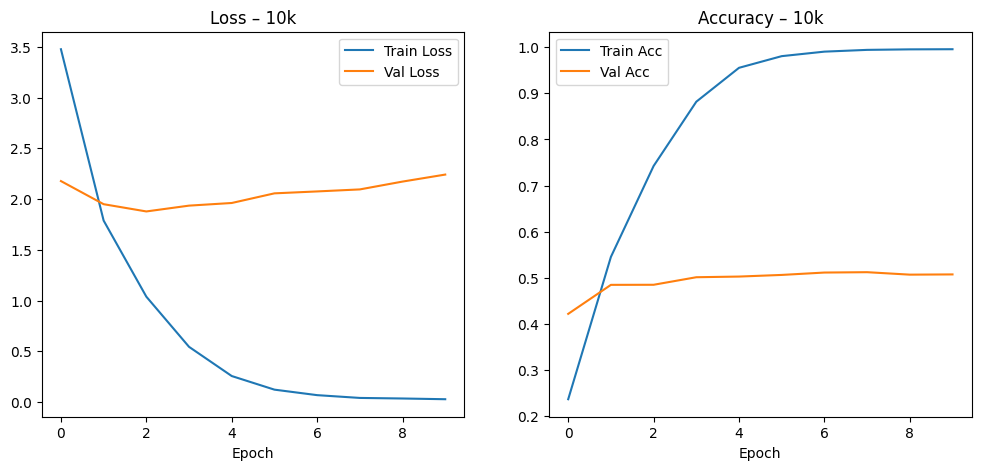
\includegraphics[width=1.0\textwidth]{images/phase03/phase03_ResNet50_10K_learning_curve.png}
    \caption{10k adathalmazon történő tanítás grafikonja Resnet50 modellen.}
    \label{fig:phase03_ResNet50_5K_learning_curve}
  \end{figure}


\subsubsection{5k adathalmazon történő tanítás eredményei.}


%25K-----------------------------------------------------------------------------
\subsubsection{25k adathalmazon történő tanítás lépései Resnet50 modellen.}


\subsubsection{25k adathalmazon történő tanítás grafikonja Resnet50 modellen.}
  \begin{figure}[H]
    \centering
    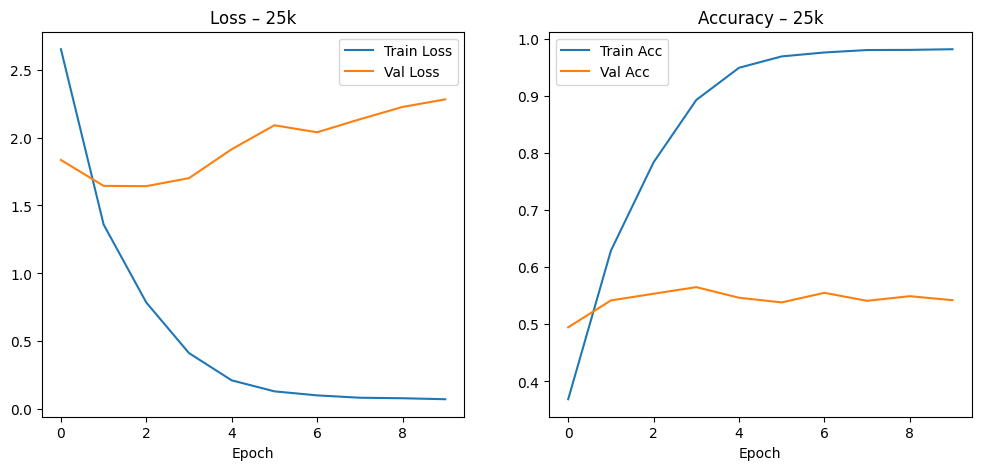
\includegraphics[width=1.0\textwidth]{images/phase03/phase03_ResNet50_25K_learning_curve.png}
    \caption{25k adathalmazon történő tanítás grafikonja Resnet50 modellen.}
    \label{fig:phase03_ResNet50_25K_learning_curve}
  \end{figure}


\subsubsection{25k adathalmazon történő tanítás eredményei.}

























\subsubsection{ResNet50 tanítás nélküli részletes osztályonkénti metrikák}
  %\begin{center}
\begin{longtable}{lllll}
\caption{ResNet50@ImageNet1k tanítás nélküli részletes osztályonkénti metrikák}\label{tab:phase1_resnet50_class_table}\\
\toprule
class & precision & recall & f1-score & support \\
\midrule
\endfirsthead
\toprule
class & precision & recall & f1-score & support \\
\midrule
\endhead
wing & 0.91 & 0.41 & 0.56 & 148 \\
warplane & 0.87 & 0.67 & 0.76 & 871 \\
stage & 0.84 & 0.63 & 0.72 & 3380 \\
groom & 0.81 & 0.23 & 0.36 & 285 \\
plate & 0.80 & 0.73 & 0.77 & 143 \\
gondola & 0.78 & 0.55 & 0.64 & 227 \\
Egyptian-cat & 0.69 & 0.73 & 0.71 & 145 \\
dock & 0.69 & 0.29 & 0.40 & 84 \\
dome & 0.67 & 0.31 & 0.42 & 85 \\
tabby & 0.67 & 0.66 & 0.67 & 107 \\
bee & 0.65 & 0.59 & 0.62 & 212 \\
electric-guitar & 0.64 & 0.62 & 0.63 & 687 \\
rapeseed & 0.64 & 0.58 & 0.61 & 77 \\
suspension-bridge & 0.64 & 0.21 & 0.32 & 127 \\
cellular-telephone & 0.62 & 0.46 & 0.53 & 104 \\
church & 0.62 & 0.23 & 0.33 & 35 \\
dragonfly & 0.62 & 0.68 & 0.65 & 75 \\
microphone & 0.62 & 0.31 & 0.41 & 596 \\
paddle & 0.62 & 0.75 & 0.68 & 93 \\
valley & 0.61 & 0.62 & 0.62 & 295 \\
hip & 0.60 & 0.50 & 0.54 & 195 \\
bubble & 0.57 & 0.29 & 0.38 & 100 \\
patio & 0.57 & 0.09 & 0.16 & 144 \\
assault-rifle & 0.56 & 0.41 & 0.47 & 91 \\
menu & 0.55 & 0.69 & 0.61 & 68 \\
obelisk & 0.55 & 0.24 & 0.34 & 95 \\
streetcar & 0.55 & 0.58 & 0.57 & 65 \\
vault & 0.53 & 0.52 & 0.53 & 104 \\
breakwater & 0.52 & 0.21 & 0.30 & 58 \\
ladybug & 0.52 & 0.12 & 0.20 & 108 \\
park-bench & 0.51 & 0.28 & 0.37 & 144 \\
daisy & 0.49 & 0.76 & 0.59 & 149 \\
lakeside & 0.49 & 0.76 & 0.60 & 801 \\
matchstick & 0.49 & 0.68 & 0.57 & 127 \\
jersey & 0.48 & 0.32 & 0.39 & 154 \\
ping-pong-ball & 0.47 & 0.32 & 0.38 & 91 \\
snowplow & 0.47 & 0.55 & 0.50 & 62 \\
swimming-trunks & 0.47 & 0.34 & 0.40 & 79 \\
triumphal-arch & 0.47 & 0.27 & 0.34 & 55 \\
monastery & 0.45 & 0.35 & 0.39 & 112 \\
binder & 0.44 & 0.38 & 0.41 & 105 \\
cabbage-butterfly & 0.44 & 0.50 & 0.47 & 101 \\
oscilloscope & 0.44 & 0.57 & 0.50 & 143 \\
suit & 0.44 & 0.65 & 0.53 & 141 \\
ear & 0.43 & 0.49 & 0.46 & 80 \\
pot & 0.43 & 0.52 & 0.47 & 254 \\
tank & 0.43 & 0.82 & 0.56 & 78 \\
birdhouse & 0.42 & 0.11 & 0.18 & 116 \\
drumstick & 0.42 & 0.27 & 0.33 & 126 \\
palace & 0.41 & 0.72 & 0.52 & 139 \\
airliner & 0.40 & 0.60 & 0.48 & 80 \\
parachute & 0.40 & 0.63 & 0.49 & 117 \\
buckeye & 0.39 & 0.24 & 0.30 & 101 \\
projector & 0.39 & 0.18 & 0.25 & 157 \\
limousine & 0.38 & 0.34 & 0.36 & 119 \\
sweatshirt & 0.37 & 0.30 & 0.33 & 80 \\
vestment & 0.36 & 0.45 & 0.40 & 69 \\
book-jacket & 0.35 & 0.40 & 0.37 & 90 \\
hay & 0.35 & 0.10 & 0.15 & 73 \\
balloon & 0.34 & 0.11 & 0.17 & 338 \\
hoopskirt & 0.34 & 0.66 & 0.45 & 135 \\
car-mirror & 0.32 & 0.13 & 0.19 & 68 \\
mobile-home & 0.32 & 0.22 & 0.26 & 83 \\
worm-fence & 0.32 & 0.59 & 0.41 & 137 \\
cannon & 0.31 & 0.40 & 0.35 & 55 \\
pier & 0.31 & 0.44 & 0.37 & 97 \\
projectile & 0.31 & 0.26 & 0.28 & 117 \\
seashore & 0.31 & 0.72 & 0.44 & 289 \\
wig & 0.31 & 0.37 & 0.34 & 70 \\
candle & 0.29 & 0.41 & 0.34 & 111 \\
crutch & 0.29 & 0.14 & 0.19 & 105 \\
drum & 0.29 & 0.39 & 0.33 & 49 \\
fountain & 0.29 & 0.27 & 0.28 & 92 \\
library & 0.29 & 0.35 & 0.32 & 74 \\
earthstar & 0.28 & 0.32 & 0.30 & 121 \\
greenhouse & 0.28 & 0.14 & 0.18 & 51 \\
restaurant & 0.28 & 0.55 & 0.37 & 141 \\
sandbar & 0.28 & 0.16 & 0.20 & 83 \\
gown & 0.27 & 0.17 & 0.21 & 66 \\
altar & 0.26 & 0.47 & 0.33 & 59 \\
mountain-bike & 0.26 & 0.38 & 0.31 & 66 \\
pole & 0.26 & 0.24 & 0.25 & 136 \\
traffic-light & 0.26 & 0.17 & 0.21 & 58 \\
barn & 0.25 & 0.08 & 0.12 & 111 \\
grand-piano & 0.25 & 0.27 & 0.26 & 63 \\
harmonica & 0.25 & 0.33 & 0.29 & 100 \\
harvester & 0.24 & 0.37 & 0.29 & 71 \\
oxygen-mask & 0.24 & 0.31 & 0.27 & 143 \\
ant & 0.23 & 0.19 & 0.21 & 95 \\
neck-brace & 0.23 & 0.23 & 0.23 & 137 \\
sax & 0.23 & 0.33 & 0.27 & 112 \\
boathouse & 0.22 & 0.35 & 0.27 & 43 \\
spotlight & 0.22 & 0.30 & 0.25 & 202 \\
cardoon & 0.21 & 0.51 & 0.30 & 55 \\
marimba & 0.21 & 0.18 & 0.19 & 79 \\
radio-telescope & 0.20 & 0.21 & 0.21 & 108 \\
bell-cote & 0.19 & 0.30 & 0.23 & 77 \\
hen-of-the-woods & 0.19 & 0.40 & 0.26 & 105 \\
beacon & 0.18 & 0.34 & 0.24 & 62 \\
mountain-tent & 0.18 & 0.06 & 0.09 & 121 \\
picket-fence & 0.18 & 0.02 & 0.03 & 118 \\
torch & 0.18 & 0.39 & 0.24 & 116 \\
missile & 0.17 & 0.26 & 0.21 & 82 \\
prison & 0.17 & 0.43 & 0.25 & 101 \\
space-shuttle & 0.17 & 0.14 & 0.15 & 84 \\
volcano & 0.17 & 0.41 & 0.24 & 119 \\
bow-tie & 0.16 & 0.04 & 0.07 & 67 \\
cinema & 0.16 & 0.18 & 0.17 & 51 \\
accordion & 0.15 & 0.30 & 0.20 & 47 \\
aircraft-carrier & 0.15 & 0.38 & 0.21 & 39 \\
theater-curtain & 0.14 & 0.62 & 0.24 & 80 \\
steel-drum & 0.12 & 0.29 & 0.17 & 84 \\
maraca & 0.11 & 0.10 & 0.11 & 90 \\
planetarium & 0.05 & 0.08 & 0.06 & 62 \\
\midrule
accuracy &  &  & 0.47 & 18172 \\
macro avg & 0.39 & 0.38 & 0.36 & 18172 \\
weighted avg & 0.53 & 0.47 & 0.47 & 18172 \\
\bottomrule
\end{longtable}
\end{center}


\subsubsection{GPU memóriahasználat}
\begin{itemize}
  \item aktív GPU: NVIDIA A100-SXM4-40GB
  \item GPU memória (lefoglalt): 0.96 GB
  \item GPU memória (használt):  0.14 GB
\end{itemize}
